% ****** Start of file apssamp.tex ******
%
%   This file is part of the APS files in the REVTeX 4.2 distribution.
%   Version 4.2a of REVTeX, December 2014
%
%   Copyright (c) 2014 The American Physical Society.
%
%   See the REVTeX 4 README file for restrictions and more information.
%
% TeX'ing this file requires that you have AMS-LaTeX 2.0 installed
% as well as the rest of the prerequisites for REVTeX 4.2
%
% See the REVTeX 4 README file
% It also requires running BibTeX. The commands are as follows:
%
%  1)  latex apssamp.tex
%  2)  bibtex apssamp
%  3)  latex apssamp.tex
%  4)  latex apssamp.tex
%
\documentclass[%
 reprint,
%superscriptaddress,
%groupedaddress,
%unsortedaddress,
%runinaddress,
%frontmatterverbose, 
%preprint,
%preprintnumbers,
%nofootinbib,
%nobibnotes,
%bibnotes,
 amsmath,amssymb,
 aps,
%pra,
%prb,
%rmp,
%prstab,
%prstper,
%floatfix,
]{revtex4-2}

\usepackage{graphicx}% Include figure files
\usepackage{dcolumn}% Align table columns on decimal point
\usepackage{esvect}% custom arrow styles
\usepackage{bm}% bold math
\usepackage{algorithm}
\usepackage{algpseudocode}
%\usepackage{hyperref}% add hypertext capabilities
%\usepackage[mathlines]{lineno}% Enable numbering of text and display math
%\linenumbers\relax % Commence numbering lines

%\usepackage[showframe,%Uncomment any one of the following lines to test 
%%scale=0.7, marginratio={1:1, 2:3}, ignoreall,% default settings
%%text={7in,10in},centering,
%%margin=1.5in,
%%total={6.5in,8.75in}, top=1.2in, left=0.9in, includefoot,
%%height=10in,a5paper,hmargin={3cm,0.8in},
%]{geometry}

\begin{document}

\preprint{APS/???}

\title{Learning Network}

\author{Roie Ezraty}
 \email{roie.ezraty@mail.huji.ac.il}
\author{Shmuel M. Rubinstein}%
\affiliation{Racah Institute of Physics, Hebrew University of Jerusalem, Jerusalem 9190401, Israel
}

\date{\today}% It is always \today, today,
             %  but any date may be explicitly specified

\maketitle

\begin{abstract}

Abstract - 

\end{abstract}

\section{Introduction}\label{sec:Introduction}

    The magic sentence: the resistance of an edge changes due to the pressure drop across it

    - The laws of physics makes a system learn by gaining energy instead of internal man-made laws that require energy

    - Can a system be trained where only its inputs and outputs are accessible, harnessing on the physical properties to change internal degrees of freedom rather than changing them by hand?

    - Cite Scellier "EqProp" PhD thesis \cite{scellier2021deeplearningtheoryneural}, and paper \cite{scellier2017equilibrium}, Altman elastic network \cite{altman2024experimental}, Dillavou laboratory demostration \cite{dillavou2022demonstration}, Stern Learning without neurons \cite{stern2023learning}, Wright, Onodera and Mcmahon deep physical with backprop \cite{wright2022deep}, Pashine, Hexner directed aging \cite{pashine2019directed}, Gold, England driven Ising model \cite{gold2019self}, Kedia, England bi-stable driven, minimal power \cite{kedia2019drive}, Berneman and Hexner on spring networks in the dynamical regime where they calculate backpropagation \cite{berneman2024designing}. constrastive (general) and coupled (physical) learning \cite{stern2021supervised}. Catastrophic forgetting of Nachi \cite{stern2020continual} and of French \cite{FRENCH1999128}. 

    - The rules for change in internal degrees of freedom are local and are constrolled by the physical laws of the problem, not by the user. We look at systems where the resistances is proportional, or changes due to, the pressure drop, flow, or power dissipation across itself, locally. 

    A key difficulty in physical learning networks is the need to store memory of the internal degrees of freedom; To address this, we suggest a scheme that trains any mechanical system that minimizes power dissipation by manipulating only the inputs and outputs. We show that a simple resistor network where resistances change due to local pressure differences can perform a) linear regression tasks and b) simple classification tasks, alluding to more efficient training and better understanding of a wide class of learning physical systems.

\section{Methods}\label{sec:Methods}


\subsection{Theoretical considerations}\label{sec:theoretical}

    We look at a general family of resistor networks where each resistor is a network edge connecting nodes $i$ to $j$ and has resistance $R_{ij}$ which are the internal degrees of freedom. The physical observables here are pressures on nodes $p_i$, but other observables can be used without loss of generality. The network automatically minimizes the total power dissipation over all edges, defined as
    
    \begin{equation}\label{eq:power_dissipation}
        \mathcal{P}=\sum \frac{\Delta p_{ij}^2}{R_{ij}} \ ,
    \end{equation}

    with respect to pressure differences on the edges $\Delta p_{ij}$. Since the network is in general not fully connected, a connectivity matrix must be constructed to calculate $\Delta p_{ij}=p_i-p_j$. Some input nodes $\vec{x}$ have pressures assigned to them externally and pressure is measured on some other, output nodes. Hence, the measured outputs of a network $\vec{y}$, given its internal degrees of freedom (i.e. resistances $R$), are a function of the posed inputs, i.e. $\vec{y}=\vec{f}\left(\vec{x}\right)$.  During measurement, the internal degrees of freedom of the system do not change, but under some regimes; e.g. once the constraints on the input and output nodes have sufficient amplitude or are applied for a sufficient time period, then the resistances change locally by the rule

    \begin{equation}\label{eq:R_afo_deltap}
        R_{ij}\left(t\right)=\gamma \Delta p^!_{ij}\left(t\right) \ ,
    \end{equation}

     where the superscripted exclamation marks state that the system is in the state where its resistances change, defined as the "dual" state and $\gamma$ a constant of proportionality. On an experimental level, this rule is a physical property of the material and can be achieved, for example, if the resistors are fluidic tubes that get continuously clogged due to pressure difference or flow across them, or if the fluid flowing in the resistors is shear-thickening. 
    
    Later, we explore cases where pressure differences change the resistance incrementally, as in $R_{ij}\left(t\right)=R_{ij}\left(t-1\right) + \gamma \Delta p^!_{ij}$, and cases where the resistance changes due to fluid flow $Q^!_{ij}=\frac{p^!_{ij}}{R_{ij}}$ or power dissipation on an edge, as in $R_{ij}\left(t\right) = \gamma Q^!_{ij}$ and $R_{ij}\left(t\right)=R_{ij}\left(t-1\right) + \gamma \mathcal{P}^!_{ij}$.

    We note that from minimization of power dissipation, the largest pressure drops in the system will occur along paths with high resistivity, since the resistance is at the denominator in equation \ref{eq:power_dissipation}, and in conjunction with equation \ref{eq:R_afo_deltap}, we emphasize that increasing the pressure drop across a resistor in the dual state will largely result in an increase in pressure drop across it during measurement.

    For a linear regression problem, the desired output is

    \begin{equation}\label{eq:task}
        \widehat{\vec{y}}=M\vec{x} \ ,
    \end{equation}

    where the hat symbol represents a desired output and $M$ some matrix of constants with dimensions $\left(\text{input}\times\text{output}\right)$. The aim is to change the resistances so that $f\left(\vec{y}\right)=M$ so that $\vec{y}=\widehat{\vec{y}}$. The loss function is hence defined as

    \begin{equation}\label{eq:loss}
        \vec{\mathcal{L}}\left(t\right)=\widehat{\vec{y}}\left(t\right)-\vec{y}\left(t\right) \ ,
    \end{equation}
    
    and is potentially non-positive and multi-dimensional with the same dimension as the output. We note that $M$ cannot obtain any arbitrary value since the outputs cannot have higher values than the inputs; It is constrained so that all the entries of $M$ sum up to less than the input values. However, if a general $M$ is desired, dividing the whole task matrix $M$ by a constant and multiplying the outputs by the same constant will yield the desired task. The relevant nomenclature for this work is given in Table \ref{tab:nomenclature}.

    \begin{table}[b]%The best place to locate the table environment is directly after its first reference in text
    \caption{\label{tab:nomenclature}%
    Relevant Nomenclature for the training scheme.
    }
    \begin{ruledtabular}
    \begin{tabular}{lcdr}
    \textrm{Notation}&
    \textrm{Meaning}\\
    \colrule
        $p$ & node pressures in all the network\\ 
        $\vec{x}$  & input pressures, dimension $d_{in}$\\
        $\vec{y}$  & output pressures, dimension $d_{out}$\\
        $R$  & Resistances\\
        $\vec{\mathcal{L}}$ & Loss, dimension $d_{out}$\\
        $\alpha$  & learning rate, scalar\\
        $\gamma$  & resistance-pressure ratio coefficient, scalar\\
        $\cdot$  & dot product\\
        $\odot$  & Hadamard (element-wise) product\\
        $\widehat{\boxed{}}$  & desired value of the task\\
        $\boxed{}^{!}$  & dual value, resistances updated using these values\\
        $\boxed{}_{i}$  & dimensions $i$\\
        $t$  & training step $\#$
    \end{tabular}
    \end{ruledtabular}
    \end{table}

    In this work, we examine a network in which each input node is connected to each output node. Moreover, each input and output node is connected to a ground node, held at a fixed pressure of $0$. This inhibits a constant drift of the voltage in the network as a whole. The training procedure, described in the following, capitalizes on a switching between the "measurement" and "dual" states of the system in order to minimize the loss in ways of changing the resistances.

\subsection{Training the network}\label{sec:training}

    At each training step, two input pressure samples $\vec{x},\,\vec{x}\,'$ are randomly drawn, and the outputs $\vec{y}=f\left(\vec{x}\right)\,,\,\vec{y}'=f\left(\vec{x}\,'\right)$ are measured. Each output yields a loss of its own $\vec{\mathcal{L}}=\widehat{\vec{y}}-\vec{y}\,,\,\vec{\mathcal{L}'}=\widehat{\vec{y}\,'}-\vec{y}\,'$ and from there the user wishes to change the resistances to decrease the loss in the next step. This is done by switching to the dual state and posing the constraints on inputs as well as outputs in the following way

    % \begin{align}
    % \vec{x}^{\,!}\left(t\right) &= \vec{x}^{\,!}\left(t-1\right)
    % +  \notag \\ \alpha\left(\vec{x}\left(t\right)-\vec{x}\,'\left(t\right)\right) 
    % & \odot \left(\vec{\mathcal{L}}\left(t\right)-\vec{\mathcal{L}'}\left(t\right)\right) \label{dual_values_x} \\
    % \vec{p}^{\,!}\left(t\right) &=  \vec{p}^{\,!}\left(t-1\right)
    % - \notag \\ \alpha\left(\vec{p}\left(t\right)-\vec{p}\,'\left(t\right)\right) 
    % & \|\vec{\mathcal{L}}\left(t\right)-\vec{\mathcal{L}'}\left(t\right)\| \label{dual_values_p}
    % \end{align}

    \begin{align}
    \vec{y}^{\,!}\left(t\right) &= \vec{y}^{\,!}\left(t-1\right)
    +  \alpha\left(\vec{y}\left(t\right)-\vec{y}\,'\left(t\right)\right) 
    \odot \left(\vec{\mathcal{L}}\left(t\right)-\vec{\mathcal{L}'}\left(t\right)\right) \label{eq:dual_values_x} \\
    \vec{x}^{\,!}\left(t\right) &=  \vec{x}^{\,!}\left(t-1\right)
    - \alpha\left(\vec{x}\left(t\right)-\vec{x}\,'\left(t\right)\right) 
    \|\vec{\mathcal{L}}\left(t\right)-\vec{\mathcal{L}'}\left(t\right)\| \label{eq:dual_values_p}
    \end{align}
    where $\alpha$ is a learning rate constant, $ \odot$ is an element-wise (Hadamard) product, $t$ is the current training step and $t-1$ is the previous. If not the resistance itself but the change in resistance changes proportionally to the pressure drop or current, i.e. 
    $\Delta R_{ij} \propto \Delta p_{ij} \, , \,Q_{ij}\, , \, \mathcal{P}_{ij}$ 
    then a slightly adjusted update rule is used, where
    $\vec{y}^{\,!}\left(t\right) = \alpha\left(\vec{y}\left(t\right)-\vec{y}\,'\left(t\right)\right)\odot\left(\vec{\mathcal{L}}\left(t\right)-\vec{\mathcal{L}'}\left(t\right)\right)$ 
    and 
    $\vec{x}^{\,!}\left(t\right) = -\alpha\left(\vec{x}\left(t\right)-\vec{x}\,'\left(t\right)\right)\|\vec{\mathcal{L}}\left(t\right)-\vec{\mathcal{L}'}\left(t\right)\|$.
    
    In the dual state, constraints are posed on input as well as output nodes and the resistances change according to a local physical law as in equation \ref{eq:R_afo_deltap}. Using this update rule for pressure constraints, the input pressure in the dual state goes down an approximated gradient of the loss and the dual output goes up the gradient, increasing the pressure difference in the path where previous increases resulted in lower loss, or vice verse. As stated in section \ref{sec:theoretical}, an increase in pressure difference in the dual values will result in a larger pressure drop across this path during measurement.
    This scheme differs from contrastive learning \cite{stern2021supervised} where each internal degree of freedom changes independently by comparing two pressure differences, here they change only due to measurements of inputs and outputs, reducing the amount of information needed during training.
    Since the resistances change every other sample taken randomly, it is in essence taking a batch size of $2$ from a dataset with an infinite number of samples. We note that the scheme works even when taking $p'\equiv0$, so only one sample is needed at every training step, essentially looking at a batch size of $1$. Iteration step $t$, on the other hand, is updated every time the resistances change and not every time a sample is taken. For clarity, the general training scheme is illustrated in a pseudocode in Algorithm \ref{training_algorithm}. 

\begin{algorithm}
\caption{Training algorithm}\label{training_algorithm}
\begin{algorithmic}
\For{$t\in \text{\# iterations}$} 
    \State sample $\vec{x},\,\vec{x}\,'$ \hfill \Comment{inputs}
    \State $\hat{\vec{y}}=M\vec{x},\,\hat{\vec{y}}\,'=M\vec{x}\,'$ \hfill \Comment{desired outputs}
    \State measure $\vec{y}, \quad \vec{y}\,'$ \hfill \Comment{meausred outputs}
    \State $\vec{\mathcal{L}}\left(t\right)=\vec{x}\left(t\right)-\hat{\vec{x}}\left(t\right),\,\vec{\mathcal{L}}'\left(t\right)=\vec{x}\,'\left(t\right)-\hat{\vec{x}}\,'\left(t\right)$ \hfill \Comment{Losses}
    \State $\vec{x}^{\,!}\left(t\right)=\vec{x}^{\,!}\left(t-1\right)+\alpha\left(\vec{x}\left(t\right)-\vec{x}\,'\left(t\right)\right)\odot\left(\vec{\mathcal{L}}\left(t\right)-\vec{\mathcal{L}}'\left(t\right)\right)$
    \State $\vec{p}^{\,!}\left(t\right)=\vec{p}^{\,!}\left(t-1\right)-\alpha\left(\vec{p}\left(t\right)-\vec{p}\,'\left(t\right)\right)\|\vec{\mathcal{L}}\left(t\right)-\vec{\mathcal{L}'}\left(t\right)\|$
    \State \hfill \Comment{dual state}
    \State measure $\Delta p^{\,!}_{ij}$ \hfill \Comment{dual state}
    \State $R_{ij}\left(t\right)=\gamma \Delta p^!_{ij}\left(t\right)$ \hfill \Comment{or other update rule}
\EndFor
\end{algorithmic}
\end{algorithm}


    
    In the following, we validate the proposed scheme with numerical simulations of general resistor networks that minimize of power dissipation with varying relations of resistance on an edge to the pressure drop across it and show that they perform 1) linear regression tasks and b) classification tasks. We further study the performance as the network size is scaled up.

\section{Simulation Results}\label{sec:results}

\subsection{Linear Regression}\label{sec:linear_regression}

    % We tested different relations between resistance of each edge to the pressure drop across it, with networks comprised of $2$ input, $1$ output and $1$ ground nodes. In all cases, the resistances converge to steady state values and the absolute values of the loss all decrease to zero in the course of training, dropping more slowly in the case where resistance changes due to power dissipation, as shown for the task
    % $x=\left[\begin{array}{cc}0.15 & 0.2\end{array}\right]\left[\begin{array}{c} p_{1}\\p_{2}\end{array}\right]$ in figure \ref{fig:different_R_update_schemes}. 
    
    % \begin{figure*}
    % \centerline{ 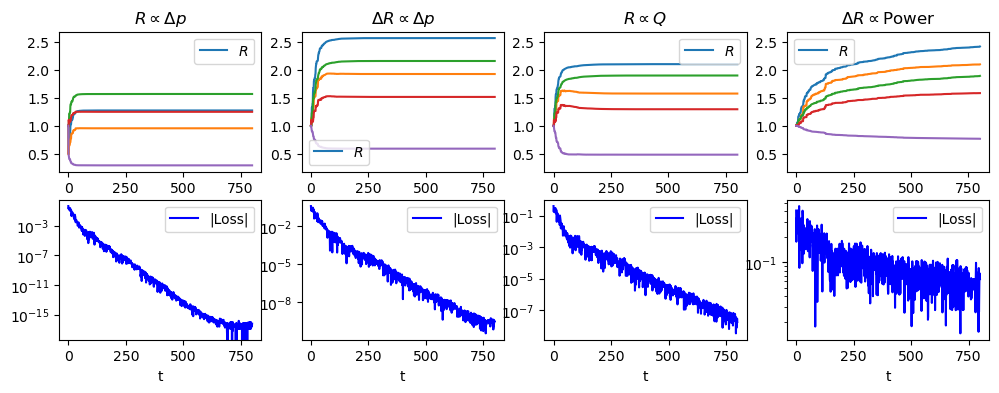
\includegraphics[width=\textwidth,height=\textheight,keepaspectratio]{Figures/different_R_update_schemes.png}
    % }
    % \caption{Resistances $R$ and absolute value of loss as function of training step $t$ for systems with different update rules for resistance, for the same training set. From left to right - $R\propto$ pressure drop on edge, change in $R\propto$ pressure drop on edge, change in $R\propto$ flow velocity through and change in $R\propto$ power dissipation on edge, respectively. In all networks the input samples during measurement were the same. All schemes show an ability to learn under sufficient amount of training steps.
    % \label{fig:different_R_update_schemes}}
    % \end{figure*}
    
    % Even though the resistances of all edges are unity at the beginning of training, the final resistances differ between the cases, so every system finds a different loss minimum in resistance space. This suggests that a vast class of physical networks can be trained to perform regression tasks using the proposed scheme, each possibly learning to perform the task in a different way. \\
    % From here on we show results only for networks whose resistances change as in equation \ref{eq:R_afo_deltap}, while they are still generalizable to other resistance change options. 
    Networks with a simple fully-connected structure, trained using our scheme, show the ability to learn tasks consisting up to $2$ inputs and $2$ outputs, to arbitrary precision. This is shown in Figure \ref{fig:variabs_in_t} where the loss decreases and resistances approach steady state values in the course of training for two example tasks.
    
    The pressure difference between inputs and outputs in the dual state exceeds that in the measured state, so during training the system is strained, in terms of inputs and outputs, beyond the task itself. This alludes to an exaggerated directed aging, in contrast to regular directed aging where a system learns as it is strained to exactly the desired amplitude and not above it.
    \begin{figure*}[ht]
    \centerline{
    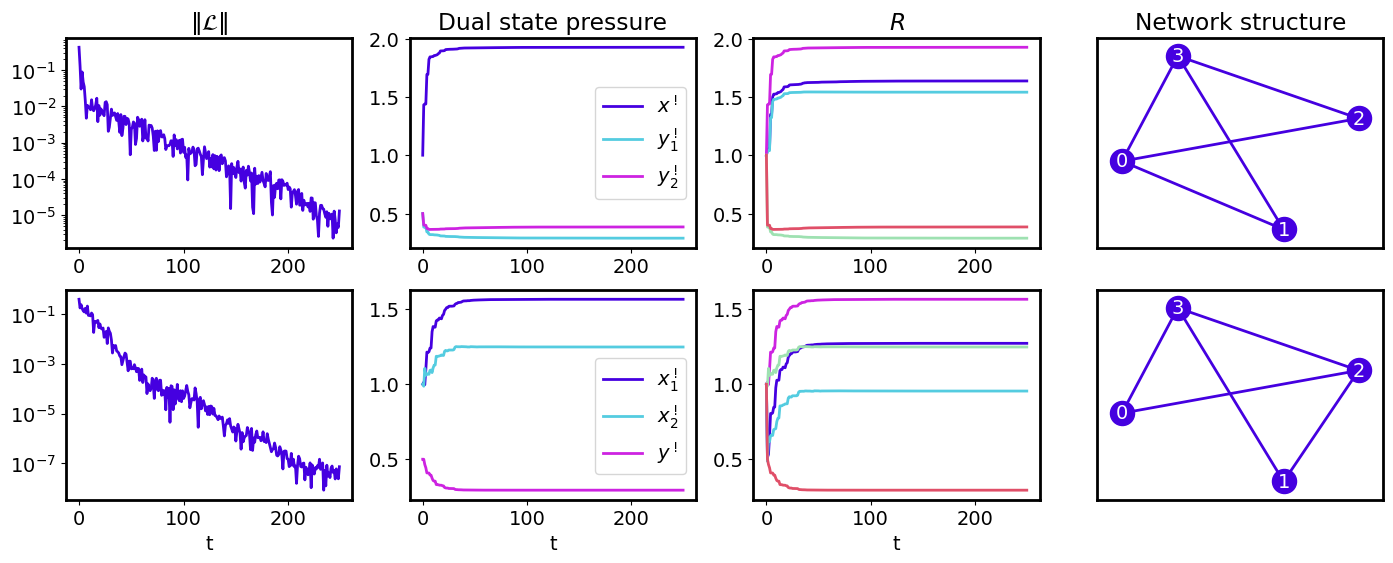
\includegraphics[width=\textwidth,height=\textheight,keepaspectratio]{Figures/performance_2_examples_4panels_mycolors.png}
    }
    \caption{Left to right - absolute value of the loss, the inputs and outputs at the dual state and the resistances as function of training step $t$, and the network structure. In the leftmost panels, the loss is normalized by the absolute value of the inputs. Upper panels show the performance of a network with $1$ input, $2$ output and $1$ ground nodes (numbered $0$ to $3$, respectively) trained for task A: $y=\left[\begin{array}{cc}0.15 & 0.2\end{array}\right]\left[\begin{array}{c} x_{1}\\x_{2}\end{array}\right]$ and lower panels for a $2$ input $1$ output and $1$ ground nodes network trained for task B: $\vec{y}=\left[\begin{array}{c}0.15\\0.2\end{array}\right]\vec{x}$.}
    \label{fig:variabs_in_t}
    \end{figure*}
    We note that the system exhibits "catastrophic forgetting" (as in \cite{FRENCH1999128}) where training the network successively task after task results in the system being able to perform only a single task at a time, erasing the memory of previous tasks once a new one is learned. Nonetheless, given every state of the system, it can be trained to perform various tasks of classification and regression, in succession.

\subsection{Classification}\label{sec:Classification}

    Classification tasks are highly non-trivial and are often a staple of versatility and generalizability for learning networks. We tested the performance of the proposed scheme on the iris benchmark dataset \cite{fisher1936use}, where one of three iris species is to be identified using $4$ input parameters. Hence, we looked at a network with $4$ input, $3$ output nodes and $1$ ground node. Instead of using a one-hot $3$ dimensional output as desired output for each iris specie, we chose the average output of all samples from the specie. This requires passing all $150$ iris samples in the dataset through the network at the beginning of each epoch and averaging over outputs from all samples of the same specie. Nonetheless, since the network is linear, this averaging is equivalent to passing the average of the inputs of that specie, which simplifies the training procedure. This averaging is essentially just tokenizing the outputs to an embedding dimension of $3$; a common practice in the field of Machine Learning. We note that the network itself specifies the desired outputs and that they converge to a steady state in the course of training. A correct classification of an iris sample is when the measured output is closest in terms of $3$ dimensional $L2$ norm to the desired output, and the accuracy of the prediction of the network is the average of samples correctly classified in the whole dataset. Using our scheme, with training set of $30$ Iris samples and the remaining $120$ are saved for test, the test accuracy easily reaches $93\%$ after less than an epoch, as in Figure \ref{fig:accuracy_vs_t}.

    \begin{figure}[ht]
    \centerline{
    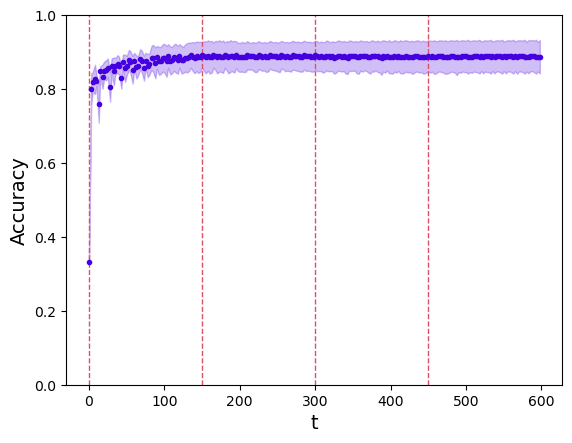
\includegraphics[width=\columnwidth]{Figures/accuracy_vs_t_markers.png}
    }
    \caption{The prediction accuracy as function of training step $t$ (blue), defined as fraction of irises correctly classified from the full iris dataset. Solid line represent the ensemble mean out of $8$ runs and opaque bounds are one standard-deviation from mean. Dashed-red lines mark times when the desired outputs were re-calculated; At the beginning of every epoch, every $150$ training steps.}
    \label{fig:accuracy_vs_t}
    \end{figure}    

\subsection{Scaling up the network}\label{sec:scaling_up}

    A difficulty arises when taking larger dimensions for $M$ in a regression task; There, the task complexity grows and the performance of the network decreases, even if the number of resistors scales with the task, as shown in figure \ref{fig:log_loss_afo_inputs_outputs}. This happens because the number of degrees of freedom needed to solve equation \ref{eq:task} is $\left(\text{inputs}\times\text{outputs}\right)$ whereas the training scheme only changes the input and output values in the dual state which are $\left(\text{inputs}+\text{outputs}\right)$ parameters; The resistances cannot acquire any arbitrary value for the family of networks studied here. Only the tasks that include $1$ input or $1$ output can be trained to arbitrarily low loss. Moreover, it is slightly harder to train a network with many outputs and few inputs than it is the opposite way around, since in the dual state two samples of inputs are taken at every time step and the inputs are changed accordingly. every input is changed  for more inputs is not the same for $n$ inputs and $m$ outputs One way of finding the dual values for inputs and outputs that will provide the closest resistances to those that actually solve the regression task is the following: first, from equations \ref{eq:power_dissipation} and \ref{eq:task} the optimal resistances that solve the task can be extracted in the form of a sparse matrix $R_{ij}^*$ and from there pseudo-inverse on the matrix will yield the pressure differences $p_i^!-x_j^!=\frac{1}{\gamma}R_{ij}^{*-1}$. Nonetheless, this null solution performs worse than a network trained using the scheme proposed in section \ref{sec:training}, as shown in figure \ref{fig:pseudo_vs_network_comparison}, suggesting that even though the network performance decreases as the task complexity increases due to limited number of adjustable degrees-of-freedom, it still outperforms non-Machine-Learning methods that have access to the same number of degrees-of-freedom.

    \begin{figure}[ht]
    \centerline{
    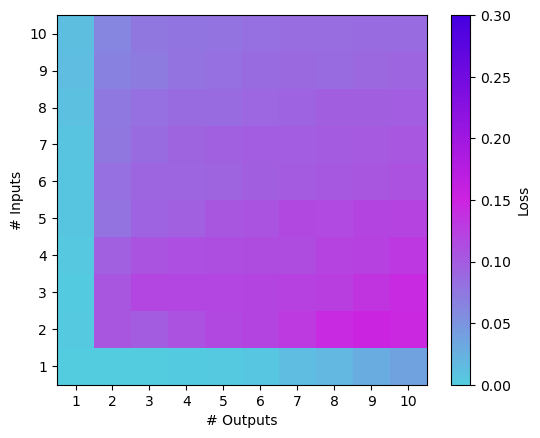
\includegraphics[width=\columnwidth]{Figures/loss_afo_in_out.png}
    }
    \caption{Normalized absolute value of the loss at final training step for tasks with varying number of inputs and outputs, denoted as $\# \, \text{Inputs}$ and $\# \, \text{Outputs}$, respectively. The normalization is with respect to the mean absolute value of the inputs over the whole dataset. Moreover, the figure present the ensemble mean over $8$ runs with randomly chosen $M$, whose entries sum up to $0.5$. The more inputs and outputs there are, the worse the model performs.}
    \label{fig:log_loss_afo_inputs_outputs}
    \end{figure}

    \begin{figure}[ht]
    \centerline{
    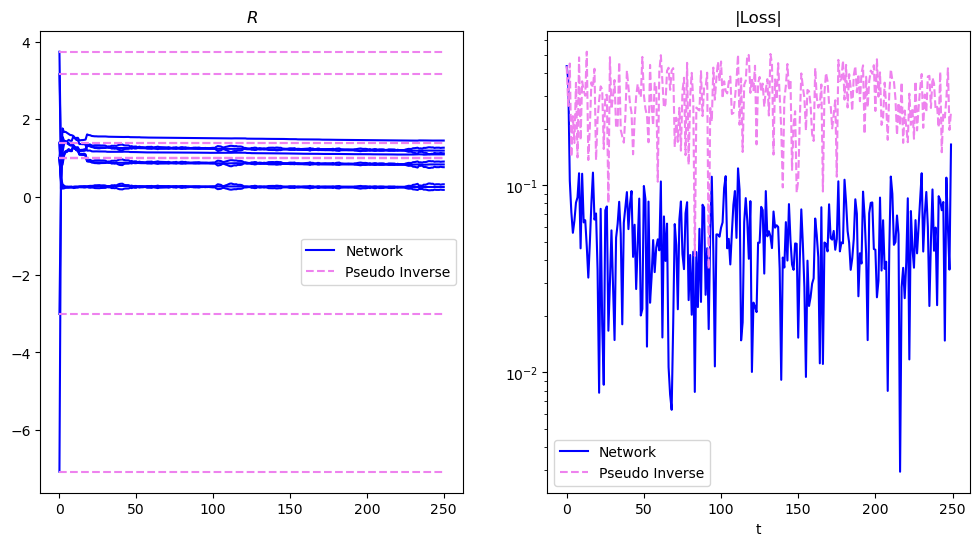
\includegraphics[width=\columnwidth]{Figures/pseudo_vs_network_comparison.png}
    }
    \caption{Comparison between resistances found using the pseudo-inverse and the ones found while training the network for an unsolvable problem of $2\text{ inputs}$ and $3\text{ outputs}$. Left panel - resistances $R$ and right panel - absolute value of the loss, as function of training step $t$. The network performs better than the null guess of the pseudo inverse, even when its resistances are initiated as identical to the ones found using pseudo-inverse.}
    \label{fig:pseudo_vs_network_comparison}
    \end{figure}

\section*{Conclusions}\label{sec:conclusions}

    In this work, we developed a novel scheme for training a broad family of physical systems to perform a plethora of learning tasks, while the only variables accessible by the user are the inputs and outputs. We have shown, by numerical simulations of resistor networks, that these systems can successfully perform a) linear regression and b) classification tasks without the need to access internal degrees of freedom. There is, however, a constraint on the regression tasks that can be performed, since the output values of a system that minimizes power dissipation and that has ground nodes are lower than the inputs. Nonetheless, a gain added to the network by way of an amplifier with a learnable amplification amplitude can expand the solvable tasks. The performance is also limited for linear regression tasks in terms of scalability of inputs and outputs, decreasing significantly for tasks that exceed $4$ parameters, but nonetheless the network trained using our method performs better than a null guess using a determinate pseudo inverse method. 
    
    The scheme harnesses the advantage of contrastive learning (cite?) where internal degrees of freedom change due to local rules solely, but differs from it since here there is no need for a twin network with constrained outputs or storage of the internal state of the whole system during each training step; Our scheme requires memory only of the input and output values. Moreover, the contrastive learning scheme requires measuring a contrast between the internal degrees of freedom in two states, whereas in ours even though the internal degrees of freedom change, there is no need to measure them, they change due to local physical relations and the system learns nonetheless. Here, internal degrees of freedom are resistances and the physical relation studied are when resistances are a function of the local pressure drop, flow or power dissipation; All three have shown ability to learn, with the relation to power dissipation being the weakest.
    
    The change of resistance rule, stated in equation \ref{eq:R_afo_deltap}, could be generalized to a broader family of materials, as in: $R_{ij}\left(t\right)=R_{ij}\left(t-1\right) + \gamma \Delta p^!_{ij}$, where the resistances have memory of their previous value, $R_{ij}\left(t\right) = R_{ij}\left(t-1\right) + \gamma Q^!_{ij}$ with fluid flow $Q^!_{ij}=\frac{p^!_{ij}}{R_{ij}}$ or $R_{ij}\left(t\right)=R_{ij}\left(t-1\right) + \gamma \mathcal{P}^!_{ij}$ with $\mathcal{P}$ the power dissipation on an edge. As shown in figure \ref{fig:accuracy_4_materials}, all $4$ rules suggested lead to learning. Even though the resistances of all edges are unity at the beginning of training, the final resistances differ between the cases, so every system finds a different loss minimum in resistance space. This suggests that a vast class of physical networks can be trained to perform regression tasks using the proposed scheme, each possibly learning to perform the task in a different way. The scheme is general enough to train different types of materials, i.e. whose resistance responds differently to the pressure distribution in the system.

    \begin{figure}[ht]
    \centerline{
    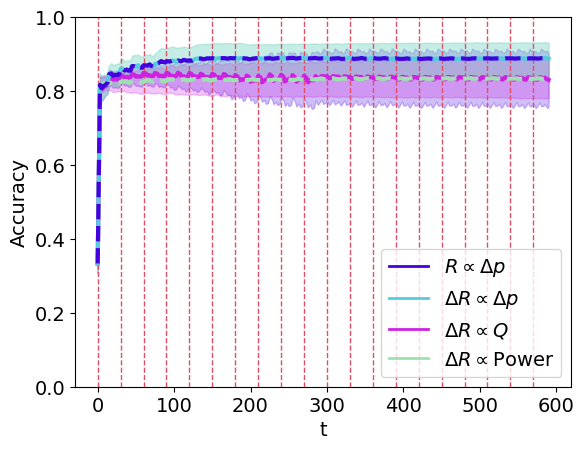
\includegraphics[width=\columnwidth]{Figures/accuracy_vs_t_4_materials.png}
    }
    \caption{Accuracy as function of training step $t$ for the Iris dataset. Here we studied $4$ systems with different change in resistance schemes, relating to $4$ different physical materials. Solid lines represent ensemble average over $8$ runs and opaque bounds are one standard deviation away from mean. dashed horizontal red lines mark times when the desired outputs were re-calculated; At the beginning of every epoch, every $150$ training steps while the accuracy was measured every $15$ training steps. All networks show the ability to learn reaching accuracy of above $80\%$ on average in less than an epoch.}
    \label{fig:accuracy_4_materials}
    \end{figure}
    
    A physical implementation of the scheme could be, for example, an electrical resistor network where resistances increase when the pressure voltage across them grows above a certain threshold. If fluidic networks are sought, pushing a fluid through tubes that clog the more flow goes through them, or that contract due to hydrostatic pressure across them, will also be trainable using our scheme. Similarly, a spring network can be harnessed by way of springs that stiffen the more they are stretched. All of the above are cheap and easily operable, and we will soon embark on implementing a physical realization ourselves.\\ 
    On the theoretical level, the learning scheme can be thought of as an exaggerated aging since in order for the system to learn, it has to be stained to values larger than those that perform the task during the state at which its internal degrees of freedom change.

    - Make sure I state both advantages: The rules for change in internal degrees of freedom are local and are constrolled by the physical laws of the problem, so learning degrees of freedom do not have to be known. Moreover there is no need for a twin for the whole networks, just for the values of the inputs and outputs to create a "dual" state.


\begin{acknowledgments}
We wish to acknowledge ???
\end{acknowledgments}

\appendix

\section{Appendix A}

???

% The \nocite command causes all entries in a bibliography to be printed out
% whether or not they are actually referenced in the text. This is appropriate
% for the sample file to show the different styles of references, but authors
% most likely will not want to use it.
\nocite{*}

\bibliography{citations}% Produces the bibliography via BibTeX.

\end{document}
%
% ****** End of file apssamp.tex ******
